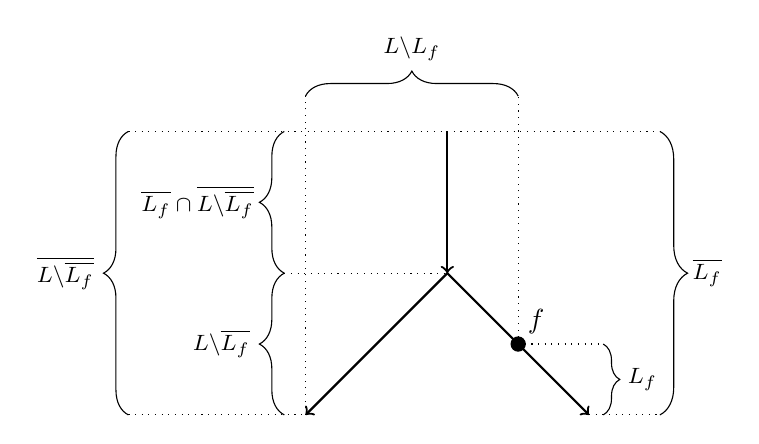
\begin{tikzpicture}[scale=.9]
% Y
\draw [thick] [->](4,5)--(4,3);
\draw [thick] [->](4,3)--(6,1);
\draw [thick] [->](4,3)--(2,1);
% Events
\draw [fill] (5,2) circle [radius=0.1];
\node [above right] at (5,2) {$f$};
% Braces
\draw [decorate,decoration={brace,amplitude=10pt}]
 	(7,5)--(7,1) node [midway,xshift=0.6cm] {\footnotesize $\overline{L_f}$};
\draw [decorate,decoration={brace,amplitude=6pt},xshift=2mm]
 	(6,2)--(6,1) node [midway,xshift=0.5cm] {\footnotesize $L_f$};
\draw [decorate,decoration={brace,amplitude=9pt}]
 	(2,5.5)--(5,5.5) node [midway,yshift=0.6cm] {\footnotesize $L\backslash
 	L_{f}$};
\draw [decorate,decoration={brace,amplitude=9pt},xshift=-3mm]
  	(2,1)--(2,3) node [midway,xshift=-8mm] {\footnotesize $L\backslash
  	\overline{L_{f}}$};
\draw [decorate,decoration={brace,amplitude=9pt},xshift=-3mm]
 	(2,3)--(2,5) node [midway,xshift=-11mm] {\footnotesize $\overline{L_f} \cap
  	\overline{L\backslash \overline{L_{f}}}$};
\draw [decorate,decoration={brace,amplitude=9pt},xshift=-5mm]
  	(0,1)--(0,5) node [midway,xshift=-8mm] 
  	{\footnotesize $\overline{L\backslash \overline{L_{f}}}$};
%Dashed lines
\draw [dotted] (5,2)--(5,5.5);
\draw [dotted] (2,1)--(2,5.5);
\draw [dotted] (6,1)--(7,1);
\draw [dotted] (5,2)--(6.2,2); 
\draw [dotted] (-0.5,5)--(7,5);
\draw [dotted] (-0.5,1)--(2,1);
\draw [dotted] (1.7,3)--(4,3);
% % Y
% \draw [thick] [->](4,2)--(4,4);
% \draw [thick] [->](4,4)--(2,6);
% \draw [thick] [->](4,4)--(6,6);
% % Events
% \draw [fill] (3,5) circle [radius=0.1];
% \node [above right] at (3,5) {$f$};
% % Braces
% \draw [decorate,decoration={brace,amplitude=10pt}]
%  	(1,2)--(1,6) node [midway,xshift=-0.6cm] {\footnotesize $\overline{L_f}$};
% \draw [decorate,decoration={brace,amplitude=6pt},xshift=-6pt]
%  	(2,5)--(2,6) node [midway,xshift=-0.6cm] {\footnotesize $L_f$};
% \draw [decorate,decoration={brace,amplitude=9pt}]
%  	(6,1)--(3,1) node [midway,yshift=-0.6cm] {\footnotesize $L\backslash L_{f}$};
% \draw [decorate,decoration={brace,amplitude=9pt},xshift=0.3cm]
%  	(6,6)--(6,4) node [midway,xshift=.8cm] {\footnotesize $L\backslash
%  	\overline{L_{f}}$};
% \draw [decorate,decoration={brace,amplitude=9pt},xshift=0.3cm]
%  	(6,4)--(6,2) node [midway,xshift=1.1cm] {\footnotesize $\overline{L_f} \cap
%  	\overline{L\backslash \overline{L_{f}}}$};
% \draw [decorate,decoration={brace,amplitude=9pt},xshift=.5cm]
%  	(7.6,6)--(7.6,2) node [midway,xshift=.8cm] 
%  	{\footnotesize $\overline{L\backslash \overline{L_{f}}}$};
% %Dashed lines
% \draw [dotted] (1,6)--(2,6);
% \draw [dotted] (1,2)--(8.1,2);
% \draw [dotted] (1.8,5)--(3,5); 
% \draw [dotted] (3,1)--(3,5);
% \draw [dotted] (6,1)--(6,6);
% \draw [dotted] (6,6)--(8.1,6);
% \draw [dotted] (4,4)--(6.3,4);

% Language L_V
% \draw [thick] [->](9,5)--(9,1);
% \draw [fill] (9,2) circle [radius=0.1];
% \node [left] at (9,2) {$f$};
% \draw [decorate,decoration={brace,amplitude=6pt},xshift=0.6cm]
%  	(9,2)--(9,1) node [midway,xshift=0.6cm] {\footnotesize $L_{V,f}$};
% \draw [decorate,decoration={brace,amplitude=9pt},xshift=0.6cm]
%  	(9,5)--(9,2) node [midway,xshift=1cm] {\footnotesize
%  	$L_V\backslash L_{V,f}$};
% \draw [dotted] (9,5)--(9.6,5);
% \draw [dotted] (9,2)--(9.6,2);
% \draw [dotted] (9,1)--(9.6,1);
\end{tikzpicture}